\section{ISO-OSI, TCP/IP}
\subsection{ISO-OSI}
Mezinárodní standard pro komunikaci po síti. Má 7 vrstev: \\
\begin{tabularx}{\linewidth}{l|l|l|l}
  \textbf{Pořadí} & \textbf{Název} & \textbf{Data} & \textbf{Pozn.}                                            \\
  \hline
  1.              & Aplikační      & Message       & Formátuje data pomocí protokolů                           \\
  \hline
  2.              & Prezentační    & Data          & Reprezentuje data a jejich zabezpečení aplikacím          \\
  \hline
  3.              & Relační        & Rel. packet   & Zabezpečuje výměnu, kontrolu, integritu a korektnost dat  \\
  \hline
  4.              & Transportní    & Segment       & Zajišťuje předání paketů správné aplikaci                 \\
  \hline
  5.              & Síťová         & Packet        & Přenos dat mezi vzdálenými počítači. Komunikace pomocí IP \\
  \hline
  6.              & Linková        & Frame         & Logické spojení na úrovni LAN. Komunikace pomocí MAC      \\
  \hline
  7.              & Fyzická        & Bit           & Fyzické spojení stran (Kabely, HW, konektory \dots)       \\
  \multicolumn{2}{l}{}                                                                                         \\
\end{tabularx}
\begin{description}
  \item[Virutální okruh -] komunikace určená cestou a nikoli adresou cíle, bez IP
  \item[Pevný okruh -] pevně sestavené administrátorem
  \item[Komutovaný okruh -] dynamicky vznikající podle potřeby
\end{description}
\subsection{TCP}
TCP/IP jsou dnes standardní protkoly pro komunikaci např. na internetu.
Má za úkol zajistit možnost propojení sítí založených na různých technologií.
Zajistit vysokou přenosovou rychlost na úkor spolehlivosti, jelikož o tu se starají koncové uzly již sami.
\begin{multicols}{2}
  Komunikace na TCP probíhá na: \\
  1. Vrstvě síťového rozhraní   \\
  2. Síťové vrstvě              \\
  3. Transportní vrstvě         \\
  4. Aplikační vrstvě           \\
  \columnbreak
  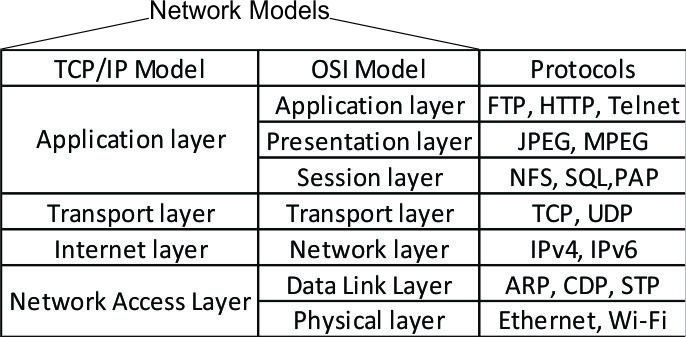
\includegraphics[height=3cm]{TVY-POS/ISO-OSI-TCP-IP/tcpip.jpg}
\end{multicols}
V koncových uzlech jsou implementovány všechny vrstvy pro kontrolu dat, v přechodových uzlech je implementována pouze síťová vrstva a vrstva síťového rozhraní.
Komunikace probíhá mezi sousedními vrstvami nebo mezi stejnolehlými vrstvami.
\begin{multicols}{2}
  Hlavička TCP protokolu:   \\
  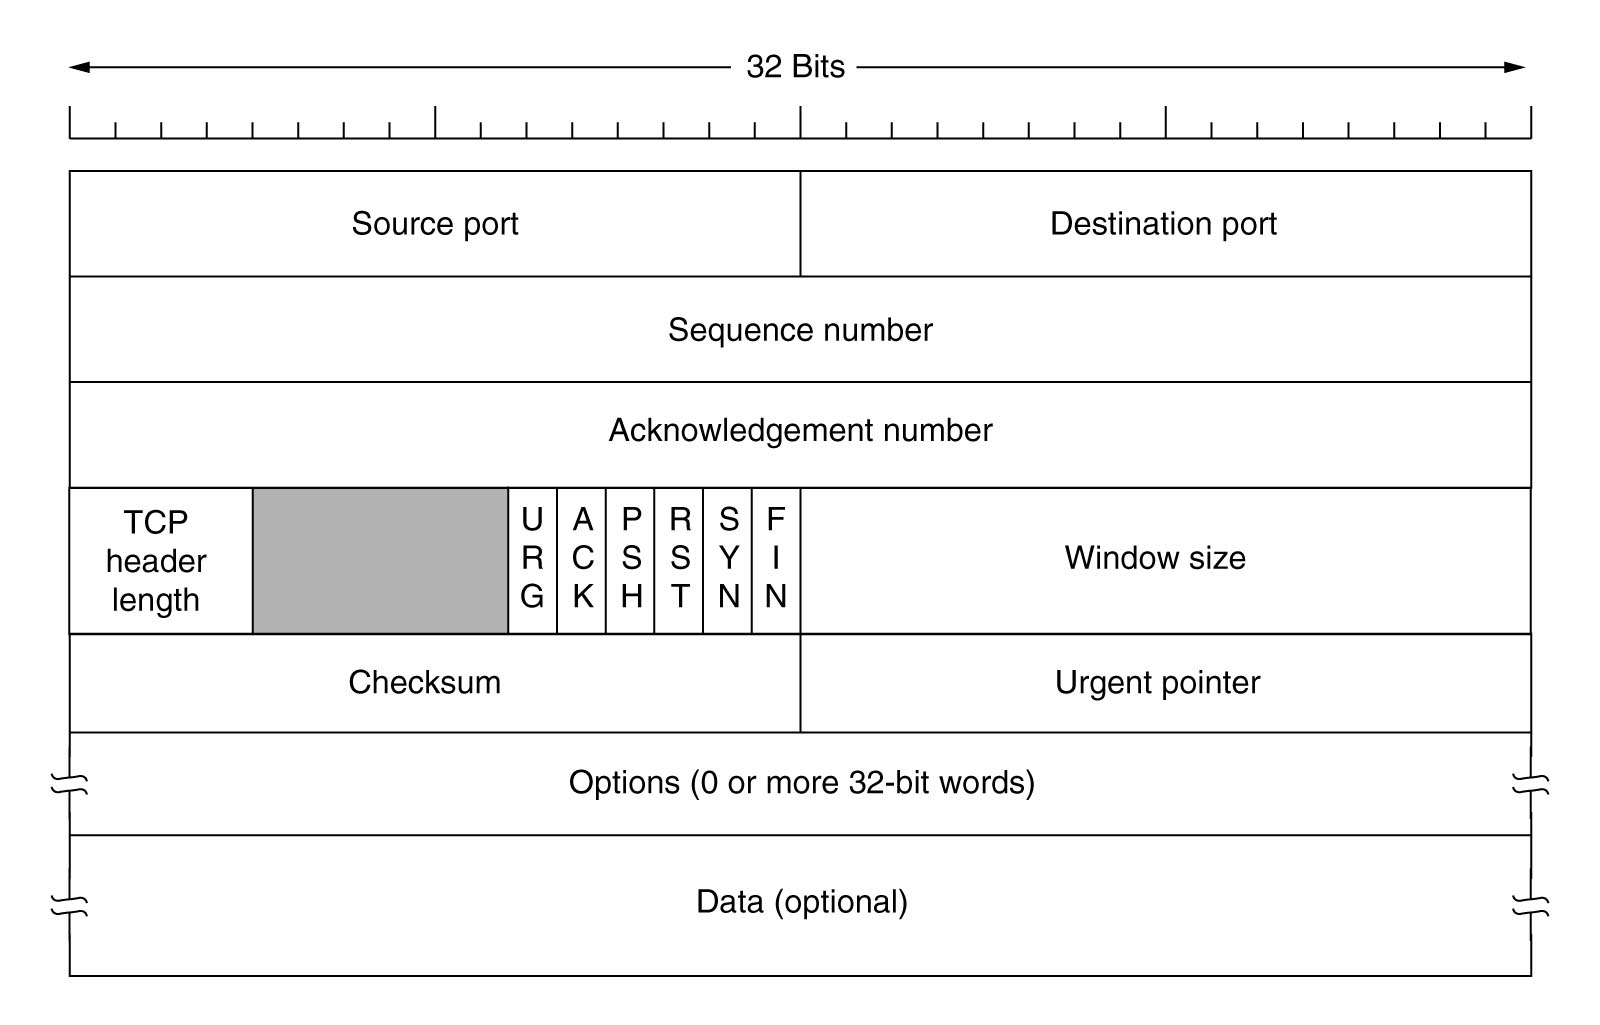
\includegraphics[width=\linewidth]{TVY-POS/ISO-OSI-TCP-IP/TCPheader.jpg}

  \columnbreak
  Pro navození komunikace:  \\
  1. Klient vyšle na server požadavek na komunikaci s příznakem SYN, náhodným číslem sekvence (x) a číslem potvrzování 0.           \\
  2. Server odešle klientovi datagram s číslem potvrzování x+1 a náhodným číslem sekvence (y), příznak zprávy nastaví na SYN, ACK.  \\
  3. Klient odešle datagram s příznakem ACK, číslem sekvence x+1, číslem odpovědi y+1.
\end{multicols}
\begin{multicols}{2}
  Hlavička UDP protokolu:   \\
  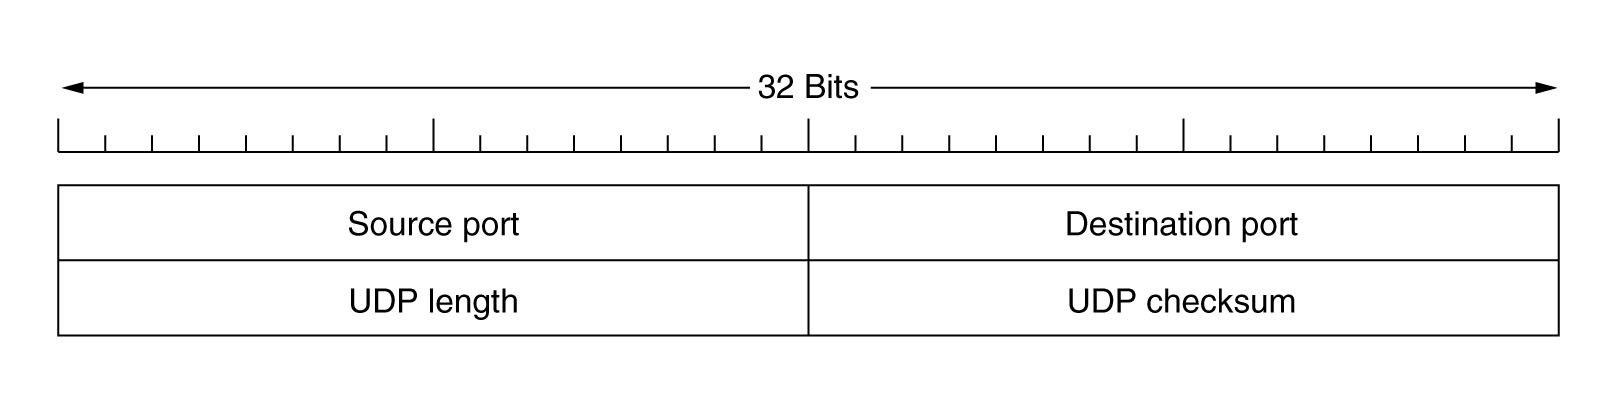
\includegraphics[width=\linewidth]{TVY-POS/ISO-OSI-TCP-IP/UDPheader.jpg}

  \columnbreak
  Pro ukončení komunikace:  \\
  1. Klient odešle FIN a příznak zprávy nastaví na FIN.  \\
  2. Server odpoví ACK a pošle FIN                       \\
  3. Klient odpoví FIN = Konec
\end{multicols}
\subsection{IP}
\begin{multicols}{2}
  Univerzální přenosový protokol k nespolehlivému, nespojovanému přenosu dat mezi zdrojovým počítačem a příjemcem.
  Každé zařízení dostává nějakou indentifikaci v podobě IP adresy.
  Přenášená data se nazývají IP datagramy neboli IP pakety, každý paket obsahuje hlavičku, ve které nese metadata a vlastní přenášená data.
  Dnes se používají protokoly IPv4 a IPv6. \\

  \columnbreak
  Formát IP diagramu: \\
  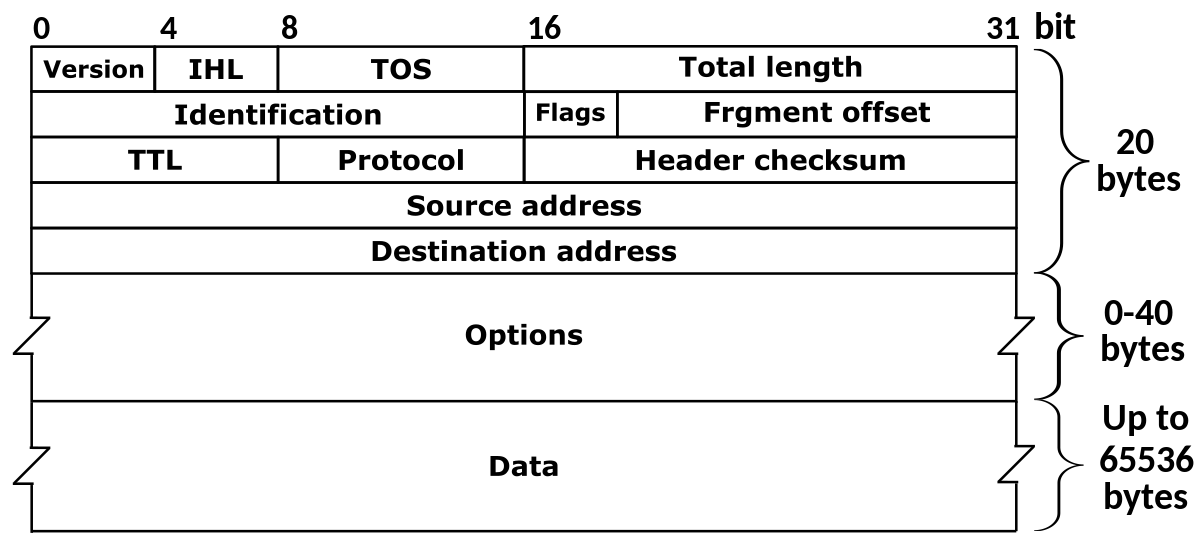
\includegraphics[width=\linewidth]{TVY-POS/ISO-OSI-TCP-IP/IPv4.png} \\
\end{multicols}
Údaje hlavičky: \\
\begin{tabularx}{\linewidth}{l|l}
  \textbf{Údaje}   & \textbf{Pozn.}                                                   \\
  \hline
  Verze            & IPv4 nebo IPv6                                                   \\
  \hline
  ToS,QoS          & Třída provozu, požadavky na přenos                               \\
  \hline
  Identifikace     & Jednoznačné určení paketu při fragmentaci                        \\
  \hline
  Příznaky         & Řízení fragmentace (more fragments, don't fragment)              \\
  \hline
  Offset           & Pozice fragmentu v původním paketu                               \\
  \hline
  Time To Live     & Položka bránící zacyklení paketu, po průchodu směrovačem snížena \\
                   & jakmile = 0 je paket zahozen                                     \\
  \hline
  Protkol          & Číslo protokolu podle RFC                                        \\
  \hline
  Kontrolní součet & Pokud nesouhlasí, je paket zahozen                               \\
  \hline
  Volby            & Doplňující informace a požadavky (obvykle se nepoužívá)          \\
  \multicolumn{2}{l}{}                                                                \\
\end{tabularx}
Pokud přenosová kapacita nestačí pro přenášená data, může IP některé pakety zahodit.
Cesta není předem vytyčena a optimální cestu nachází každý uzel, přes který daný paket jde.
Zpráva rozdělená na několik paketů nemusí dorazit ve stejném pořadí, jako byla poslána.
Každý poškozený paket síťová vrstva zahodí.
Požaduje-li aplikace spolehlivý přenos dat, jsou k dispozici protokoly vyšších vrstev.
Při přenosu velkých dat se mohou data fragmentovat.
Fragmentují se na vysílající stanici a defragmentují na přijímací.
\subsection{IEEE}
Institut pro elektrotechnické inženýrství.
Je to mezinárodní organizace zabývající se výrobou standartů v oblasti průmyslu.
Příklady protkolů: \\
\begin{tabularx}{\linewidth}{l|l}
  \textbf{Číslo} & \textbf{Pozn.}                                                                              \\
  \hline
  802.1q         & pro Trunk komunikaci VLAN                                                                   \\
  \hline
  802.3          & pro technologie Ethernetu - realizuje 1. a 3. vrstvu modelu ISO, nahrazuje Token Ring       \\
  \hline
  802.5          & pro Token Ring - technologie pro LAN, kdy předává vysílací právo pomocí rámce Token         \\
  \hline
  802.11         & WiFi - wireless fidelity - popisuje bezdrátovou komunikaci, náchylný na rušení, menší dosah \\
\end{tabularx}